\section{Introduction}

This thesis describes a possible design and a proof-of-concept implementation of a data layer for near real time distributed collaborative applications targeted at operational workloads in small to medium sized businesses with strict auditability requirements.

\paragraph{Context.} The ideas presented in this work are based on the author's experience running a \gls{SaaS} business developing and operating a highly available information system in the medical sector for the past five years (see~figure~\ref{fig:rosalind}). The deployed system covers all of the daily operational needs of medium-sized practices, handling medical records, personal data, and associated imagery for more than 80.000 patients a year, scheduling appointments, employees, departments, and rooms subject to complex business rules constraining available treatments, forecasting, planning and reporting clinical workload, sending appointment reminders, handling inbound calls and messages from patients, recording internal referrals and escalations, along with support for distributed staff (e.g. external call centers, telemedicine) owing to fine-grained roles and authorization controls, thorough audit logging of all changes, and compliance with relevant regulations.

\begin{figure}[!ht]
  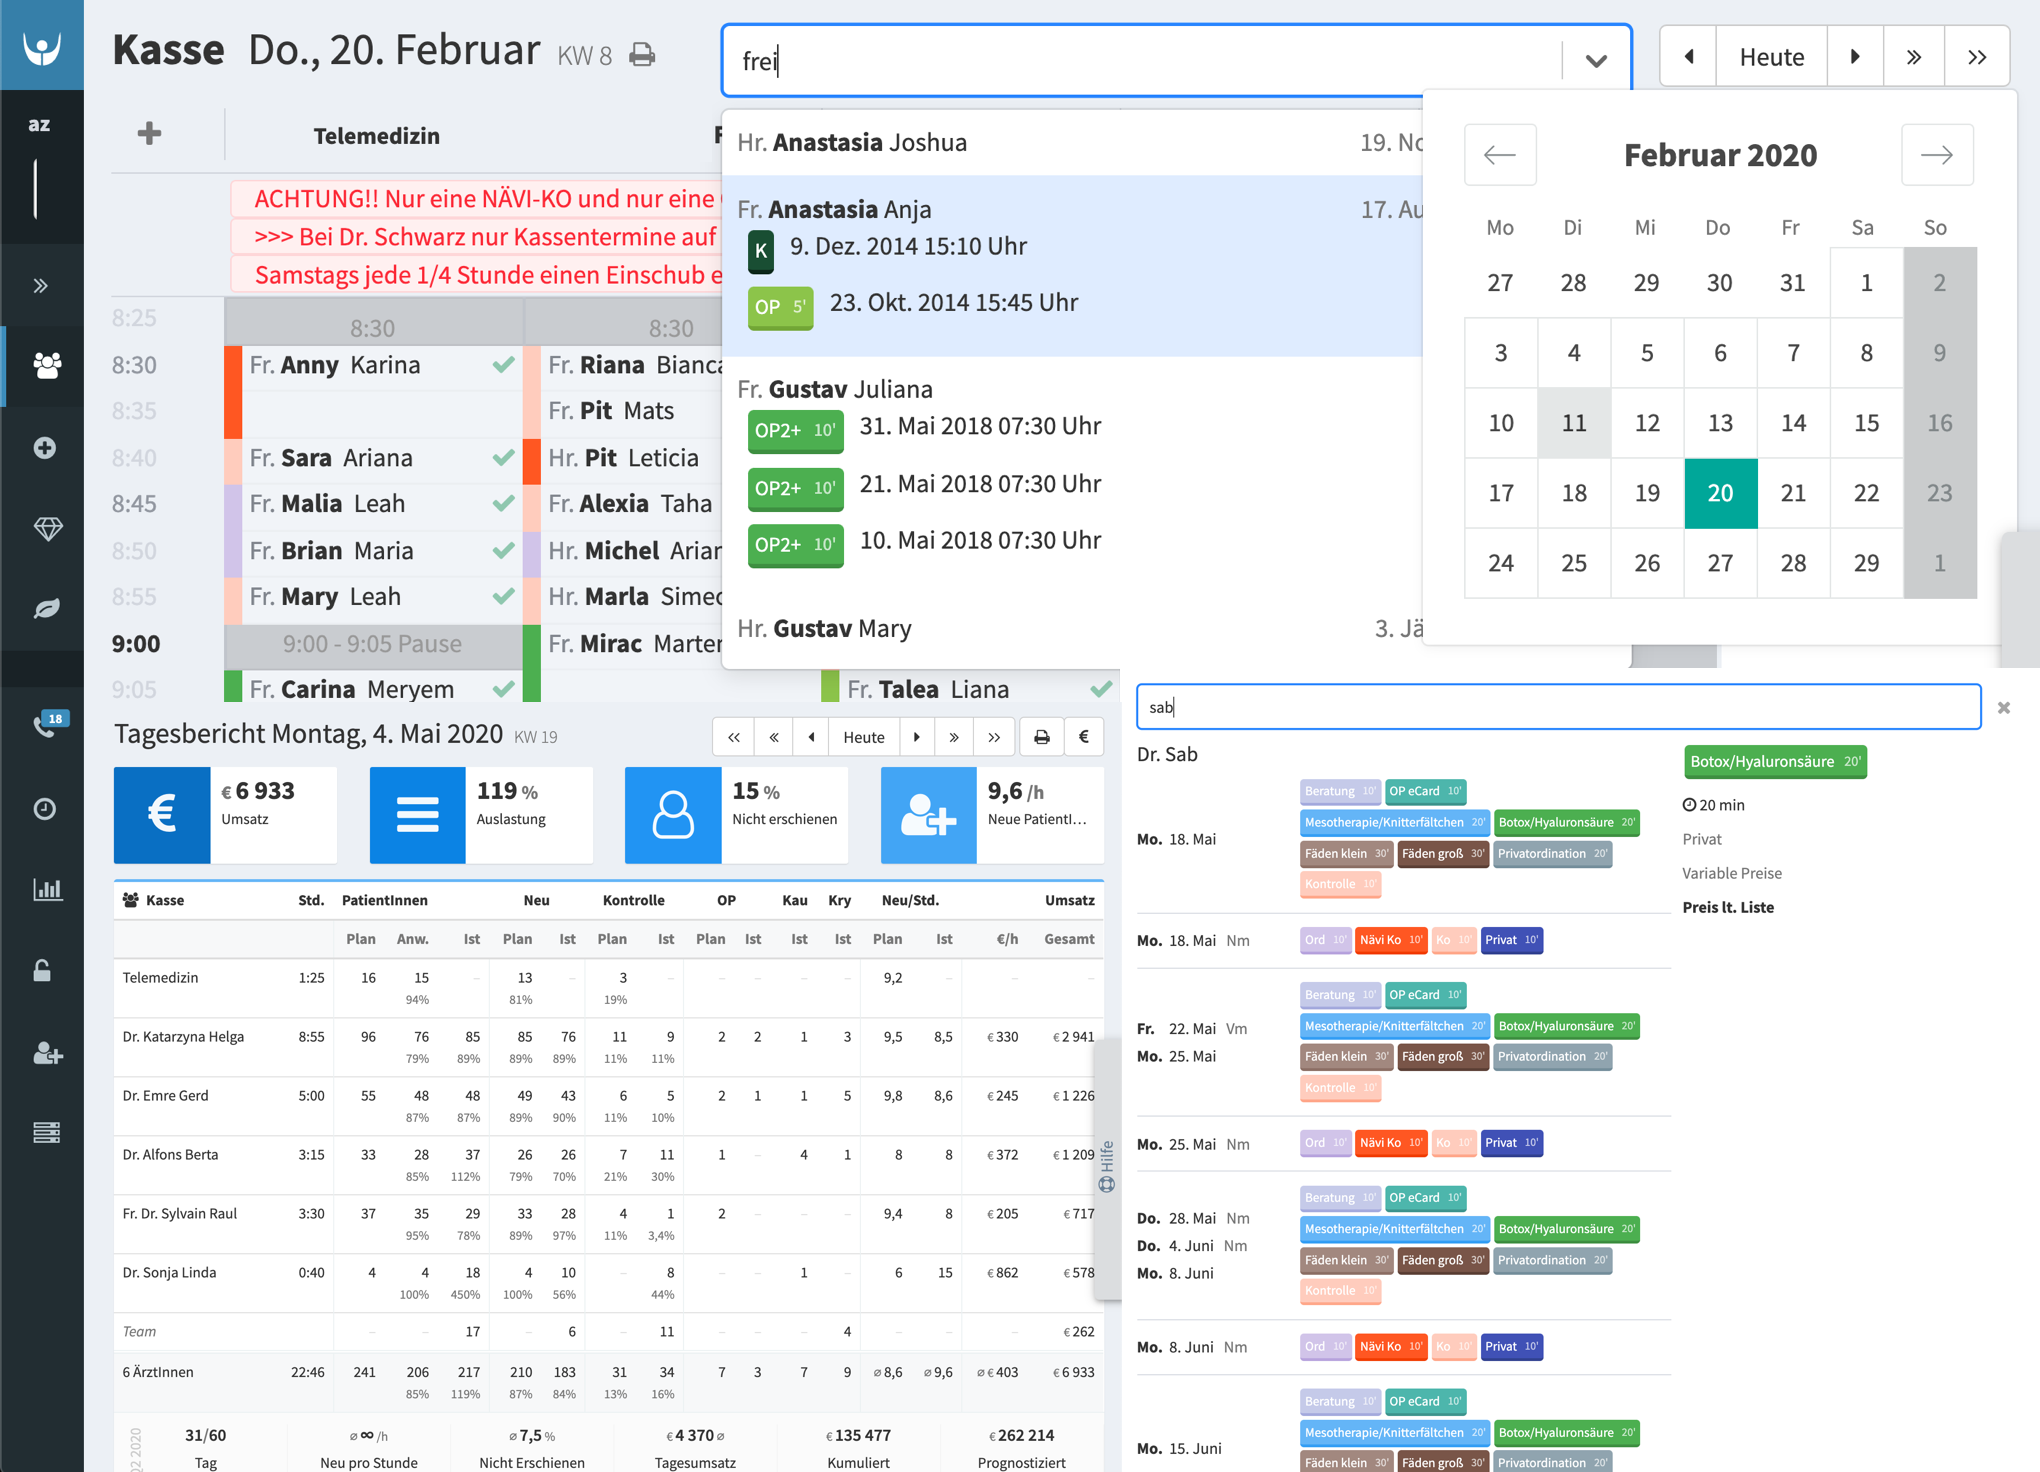
\includegraphics[width=\linewidth]{images/rosalind.png}
  \caption{The author's medical information system}
  \label{fig:rosalind}
\end{figure}


\cleardoublepage

\paragraph{Background.} The system is built on top of the open source Meteor framework (presented in section~\ref{sec:related_work}) and MongoDB, making heavy use of their "live query" mechanisms, along with Redux, React and Minimongo in the front end, packaged with Electron and React Native. To increase availability, the back end is deployed over three data centers using primary-backup replication. Currently, the tracked code base comprises about 42.000 lines of JavaScript. Being a system designed, developed, and operated by a single person, the primary challenge by far has been to keep runaway incidental complexity at bay. While the abstractions around "live" publication/subscription provided by the Meteor framework turned out to be very expressive, other design decisions of the underlying framework and database caused unnecessary complexity in the application code. Drawbacks include pervasive mutability, the need to denormalize data, the lack of a relational query language, no server-side joins, and no (bi-)temporality or notions of time or memory for auditing purposes.


\paragraph{Outline.} Section~\ref{sec:related_work} presents related work. Section~\ref{sec:design} exhibits common problems experienced in data-intensive business applications and shows a different approach towards solving some of them in a functional, immutable, and reactive way. A proof-of-concept implementation is described in section~\ref{sec:implementation} and its merits and deficiencies are discussed in section~\ref{sec:discussion}.

\cleardoublepage

\subsection{Problem}
Classic Relational Database Management Systems (RDBMS) are not suitable for modeling sparse, hierarchical or multi-valued data in domains where evolution and dynamism are hard requirements. They also lack a notion of memory or change over time because writes are destructive by default. Attempts to add concepts of temporality to Structured Query Language (SQL) are complicated and as a result not widely used. Auditing changes to a mutable black box with no history is hard. Developers fear the networking aspects of sending queries on a round trip "over there" \cite{hickey2012dbvalue} to the database, as opposed to having the data in memory and being able to query it directly. On top of all, customers demand increasingly interactive distributed collaboration environments, which pushes the limits of established request-response mechanisms.

\subsection{Contribution}
This thesis explains a possible design of a data layer for business applications and describes its prototypal implementation. The core is a simple relational data model based on facts in the form of Entity-Attribute-Value (EAV) tuples similar to the \gls{6NF} or the \gls{RDF} as seen in Semantic Web literature. Such EAV tuples are accreted in an append-only (immutable) log as assertions and retractions together with two timestamps: \gls{tx} at which the fact was added to the log, and \gls{tv} at which the fact became true in the wider context of the system \cite{snodgrass1992temporal} i.e. the real world.


\paragraph{Goal.}
The original goal of this work was to demonstrate the feasibility of an implementation of various desirable data layer features in less than 1000 lines total of readily comprehensible Lisp (Clojure, more specifically ClojureScript \cite{hickey2008clojure}): Bitemporality, practically immutable audit logging, transaction metadata, server-client reactivity, schemalessness, consistency criteria, derived facts, versatile indexing, transactions with guarantees of \gls{ACID}, and a simple relational query language based on Datalog.

\paragraph{Method.}
The thesis explains the decisions made while iterating on the design and its implementation and includes a discussion on limitations and advantages.

\paragraph{Results.}
Embracing the EAV+$t_x$+$t_v$ data model together with the expressive programming language ClojureScript reveals that it is possible to implement a proof-of-concept data layer and query language for business applications with various valuable features not commonly seen in mainstream databases. The implementation is realized using less than 400 lines of code, the majority of which appears to map fairly well to the conceptual design.
